% Chapter 6

\chapter{Event Plane} % Main chapter title

\section{Determination of Event Plane}

\begin{figure}[htbp!]
  \centering
    \begin{subfigure}[p]{0.7\textwidth}
    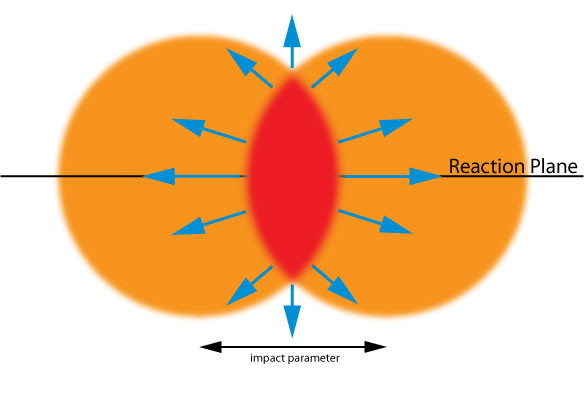
\includegraphics[width=1\textwidth]{Figures/Flow_Plane.jpg}
    \caption[Diagram showing impact parameter versus $N_spectators$ and $N_participants$]{Two dimensional representation of the event/reaction plane. Recall the impact parameter is the distance between the two colliding ions' centers. In this illustration the orange spheres represent the ions, one is going into the page and one is coming out of and the red overlap is the matter created by the participant nucleons.
    \label{fig:cernfireball}}
    \end{subfigure}
    \begin{subfigure}[p]{0.7\textwidth}
    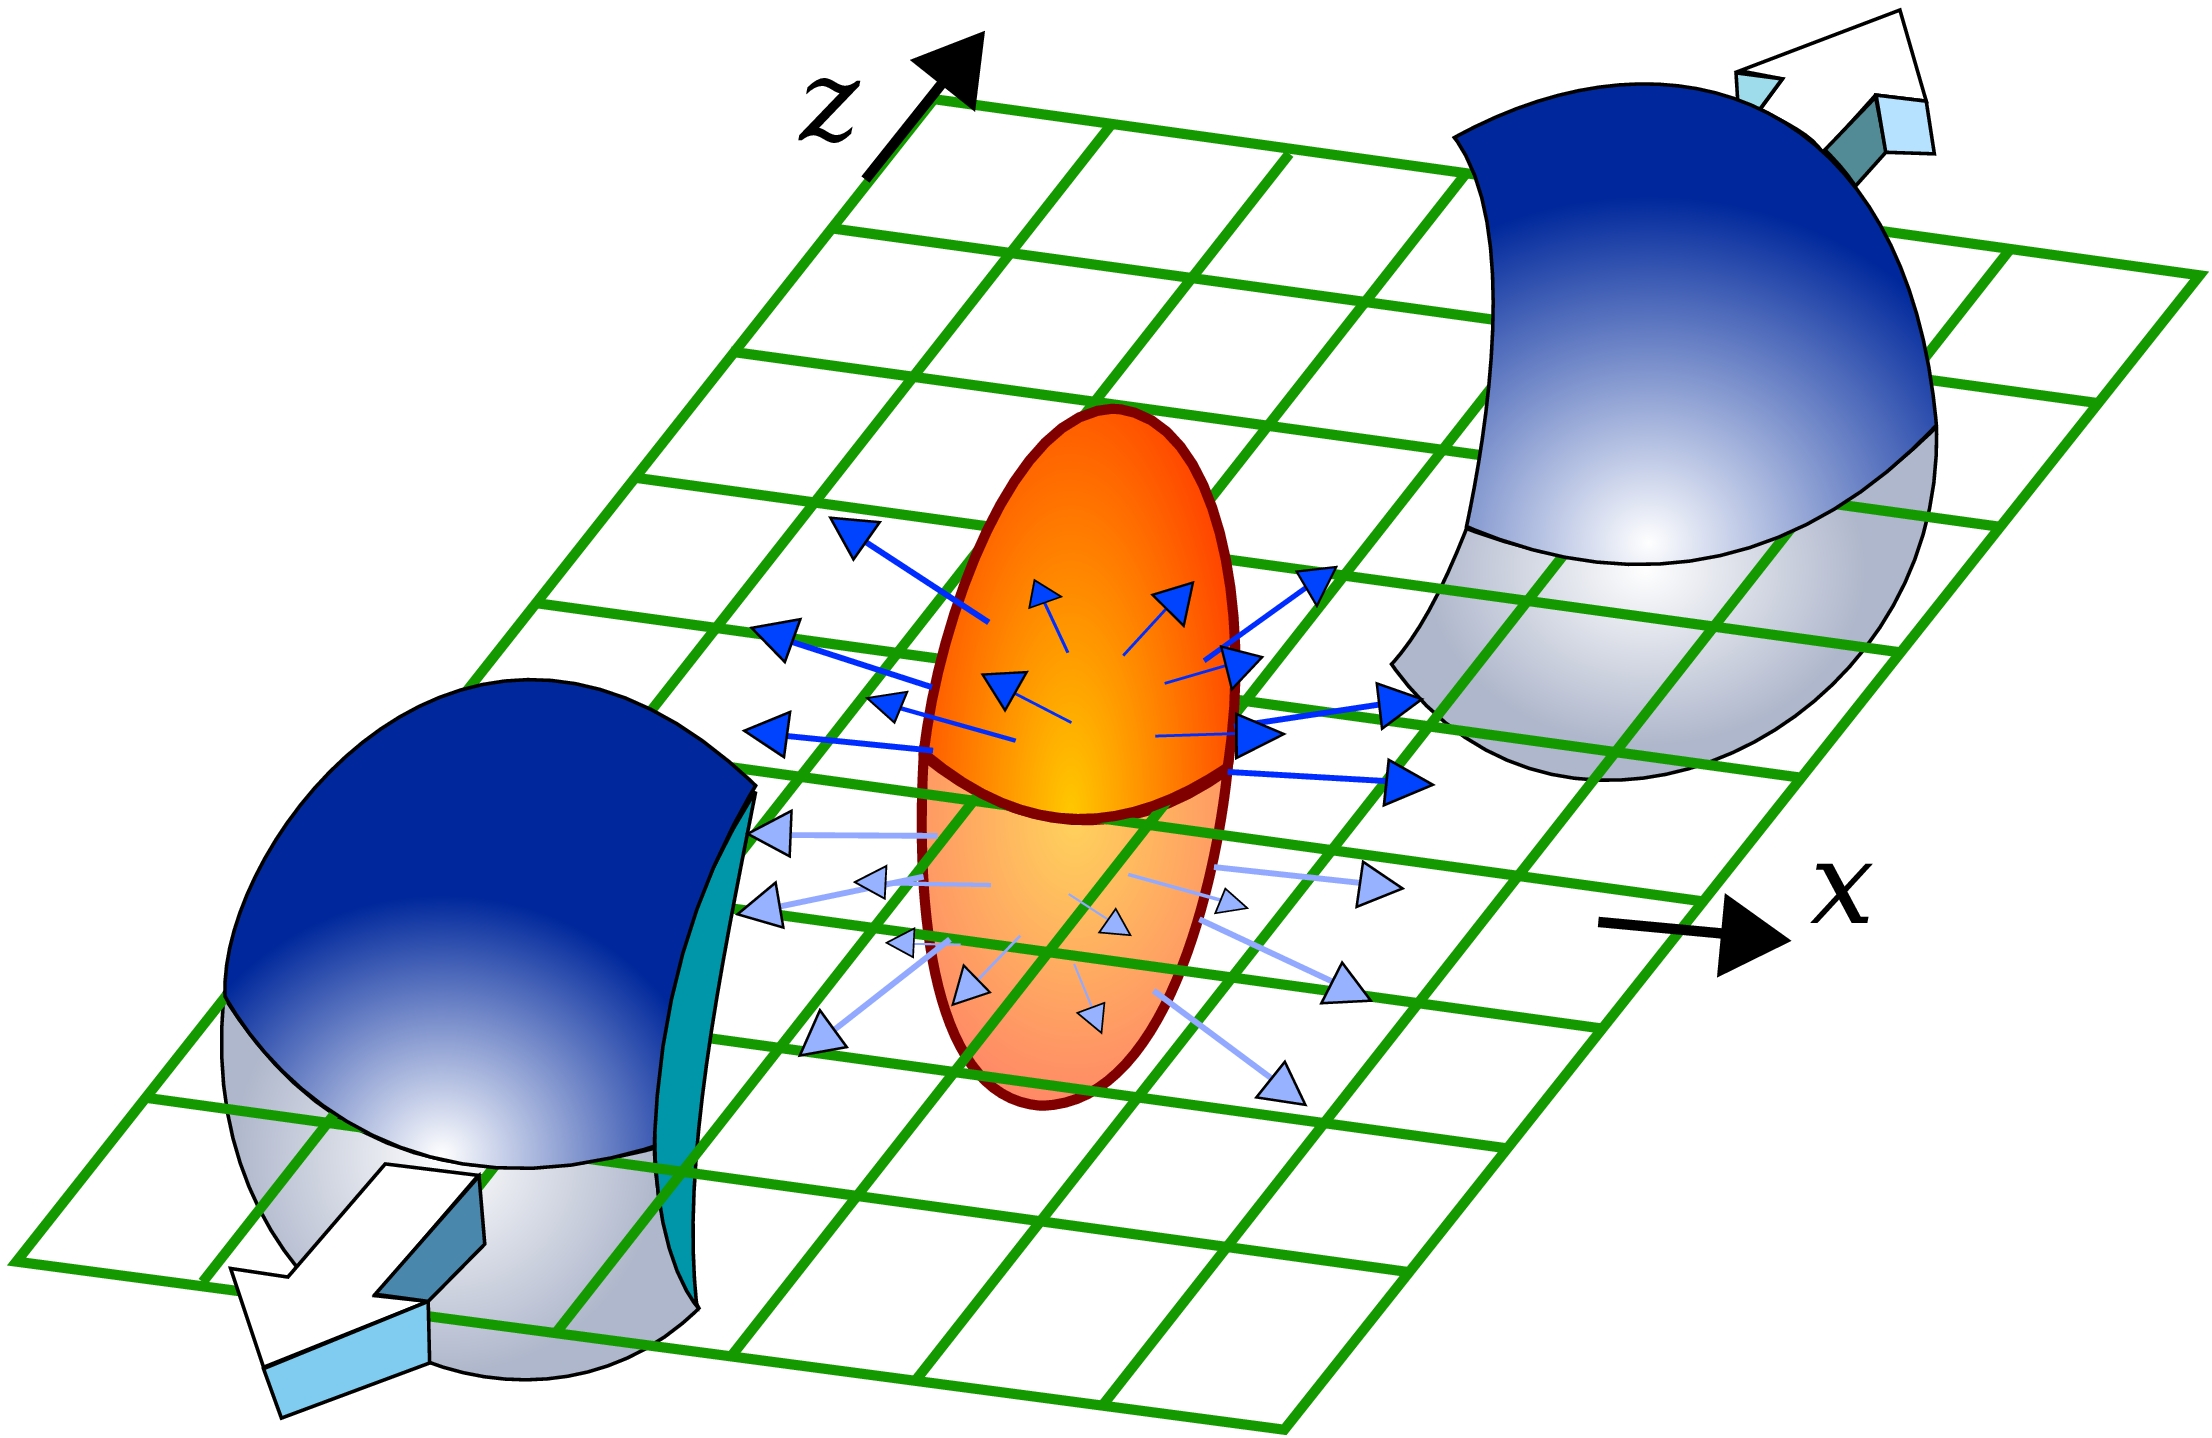
\includegraphics[width=1\textwidth]{Figures/flowcartoon.jpg}
	\caption[Central vs Peripheral collisions, geometry of initial conditions]{A three dimensional render of the initial conditions just after a collision. The two blue spheres are the remnant spectator nucleons from the colliding ions, the orange/yellow ellipsoid is the nuclear matter created by the collision of participant nucleons. The green grid here represents the plane that bisects all three of these bodies which we call the event plane}
    \end{subfigure}
    \rule{35em}{0.5pt}
  \caption[Illustrations of the event plane in heavy ion collisions]{Illustrations of the event plane in heavy ion collisions}
  \label{fig:evtpln}
\end{figure}

Pivotal to this analysis is the ability to determine an event characterization variable called the \textit{Reaction} or \textit{Event Plane}. Given the geometry of a heavy ion collision, we define the event plane as the two dimensional plane that bisects both ions equally through their centers as shown in \ref{fig:evtpln}. If we recall that the impact parameter is the distance between the two colliding ions' centers and we were to create a vector from this distance and we have a vector that represents the direction one of the ions is traveling down the beam axis, the plane containing both of these vectors is the Reaction/Event plane (it is irrelevant which direction the impact parameter vector points and which direction we pick to point the beam axis vector, this is merely for creating a plane).

In practice this plane is determined by detecting the spectator nucleons or high multiplicity track signals at high rapidity using a detector with full azimuthal coverage. Ideal candidates for this are the BBC, the SMD, and the RXNP. Particle signals would appear in the Northern detector as a cluster of hits on one side in azimuth and in the Southern detector as a cluster of hits 180$^\circ$ azimuthal degrees across. The event plane can therefore be constructed using the locations of these signal clusters and creating a plane that bisects them (see fig. \ref{fig:rxnpexpcartoon}).

\begin{figure}[htbp!]
  \centering
    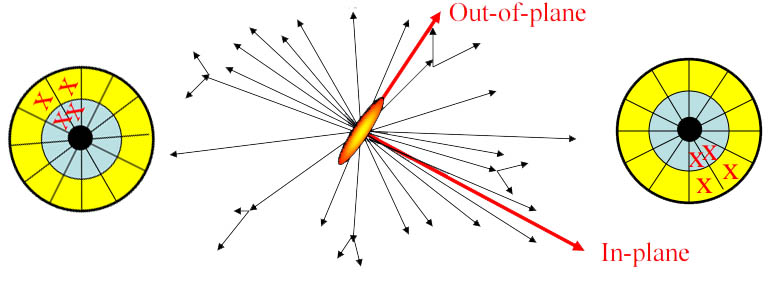
\includegraphics[width=1\textwidth]{Figures/reactionplaneexpcartoon.jpg}
    \rule{35em}{0.5pt}
  \caption[Cartoon of Event Plane determination with forward detectors]{Cartoon of Event Plane determination with forward detectors \citep{RXNPfocus}}
  \label{fig:rxnpexpcartoon}
\end{figure}

\section{Event Plane ``Flattening"}
Since we have little control over the precise impact parameter and event plane orientation for each collision, instead, data is taken and event plane orientations populate a distribution statistically and this distribution is non uniform. The process of making this distribution uniform in azimuth is called \textit{flattening}.

\begin{figure}[htbp!]
  \centering
    \begin{subfigure}[p]{0.4\textwidth}
    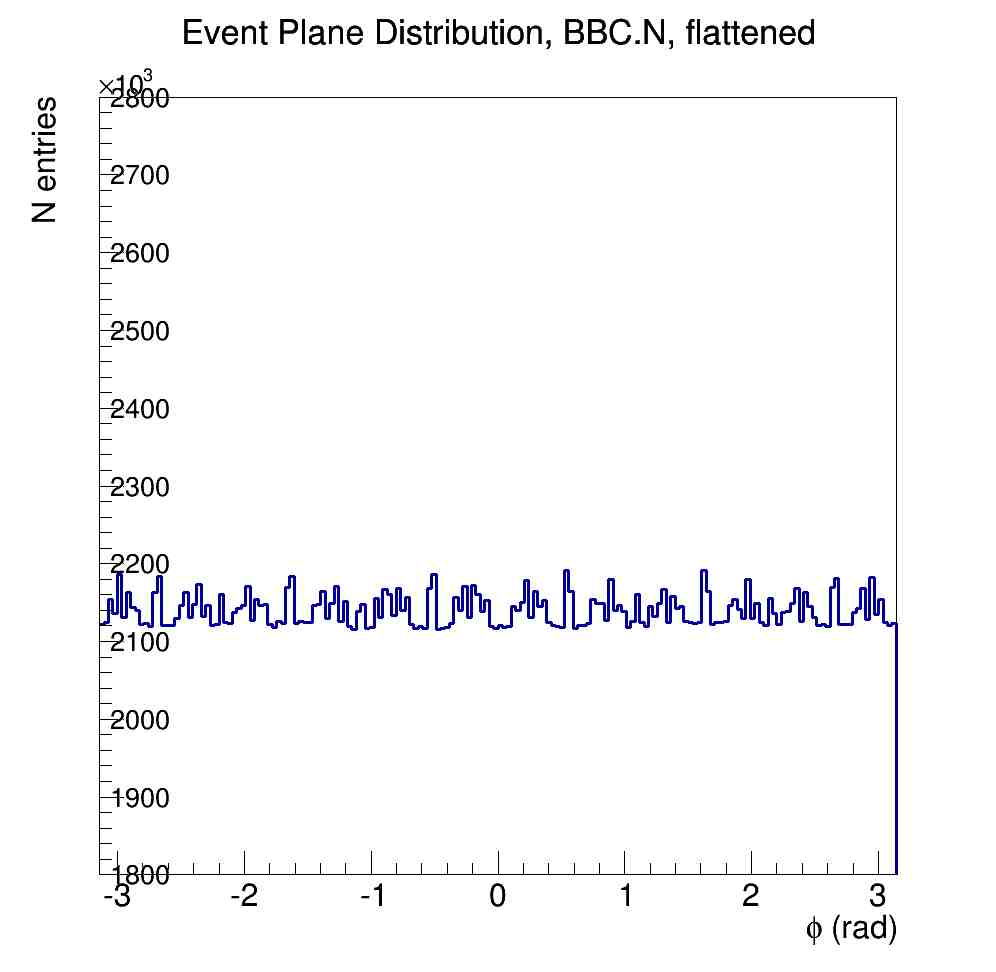
\includegraphics[width=1\textwidth]{EPflattening/flatbbcn.jpg}
    \end{subfigure}
    \begin{subfigure}[p]{0.4\textwidth}
    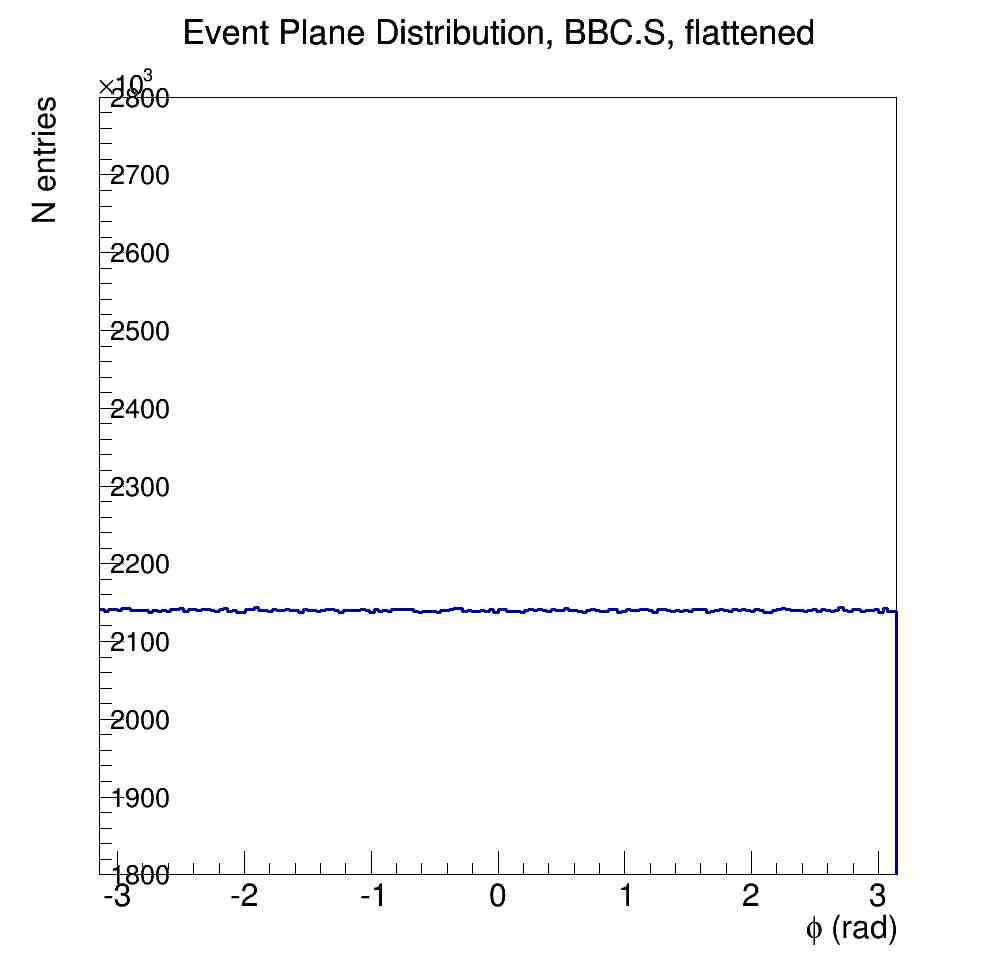
\includegraphics[width=1\textwidth]{EPflattening/flatbbcs.jpg}
    \end{subfigure}
    \begin{subfigure}[p]{0.4\textwidth}
    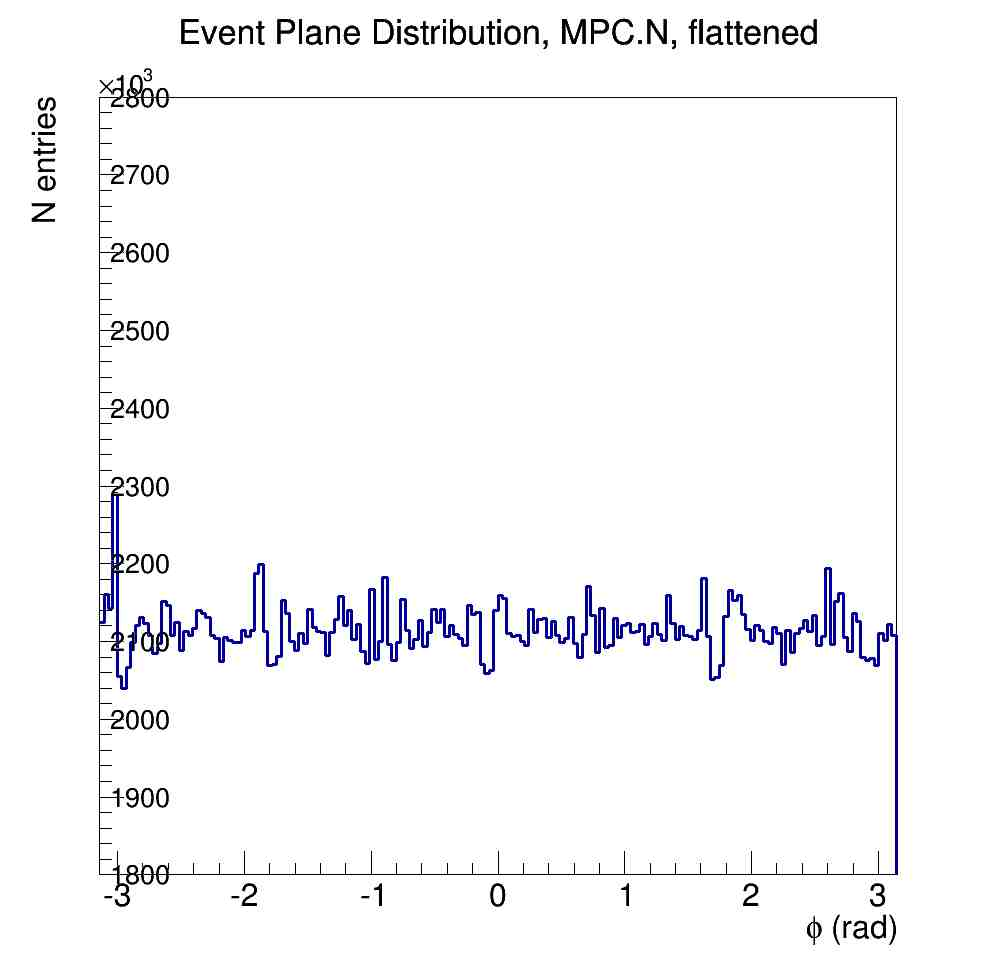
\includegraphics[width=1\textwidth]{EPflattening/flatmpcn.jpg}
    \end{subfigure}
    \begin{subfigure}[p]{0.4\textwidth}
    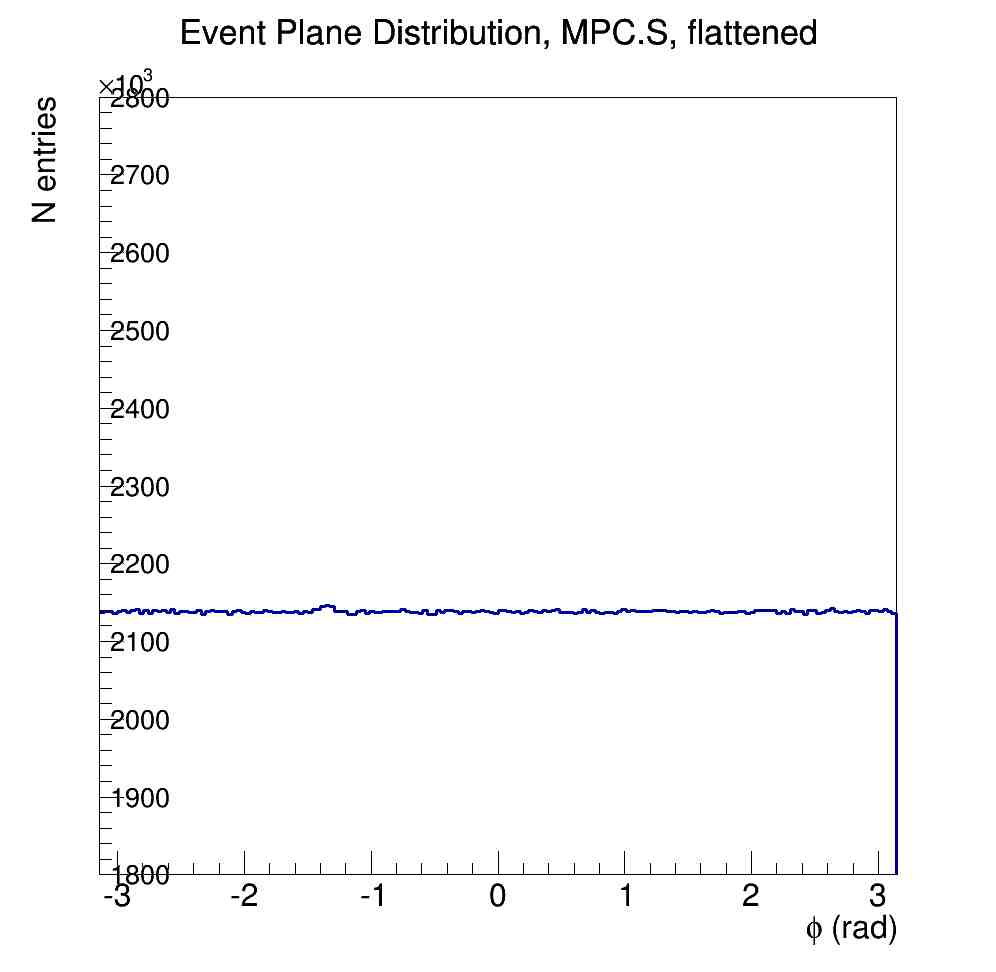
\includegraphics[width=1\textwidth]{EPflattening/flatmpcs.jpg}
    \end{subfigure}
    \begin{subfigure}[p]{0.4\textwidth}
    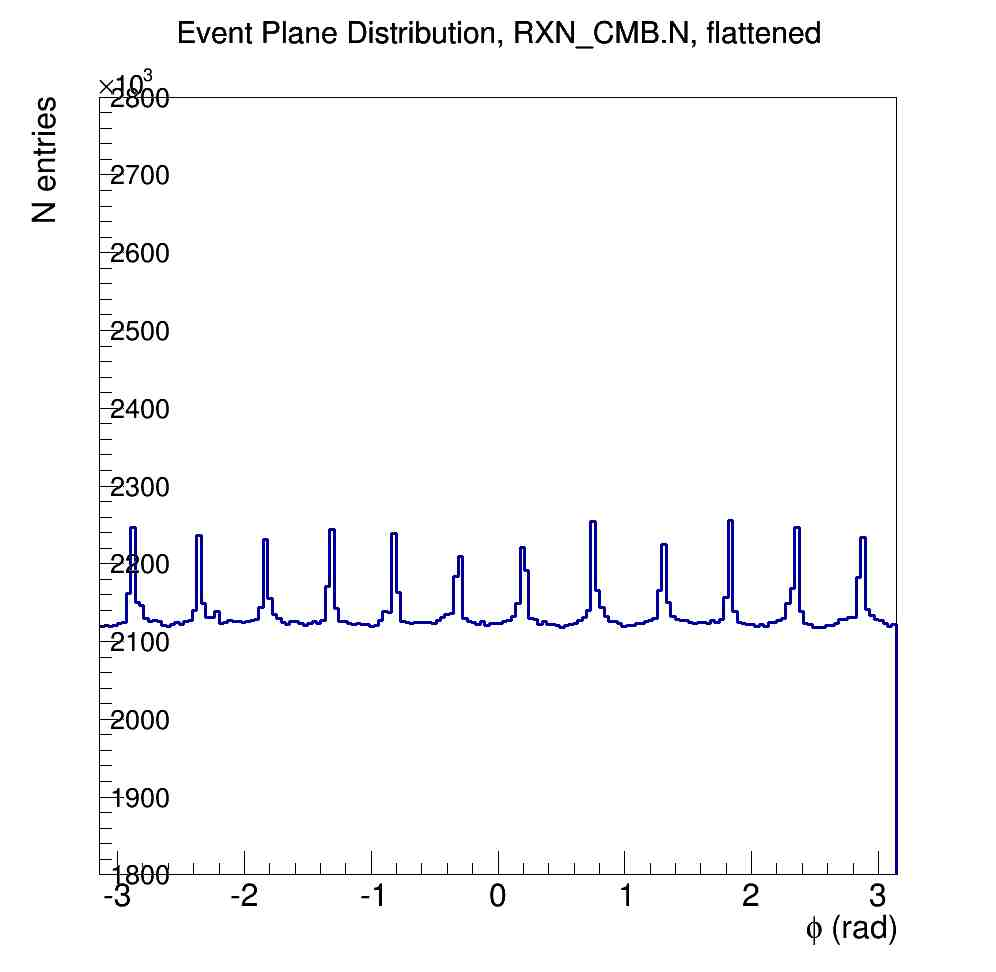
\includegraphics[width=1\textwidth]{EPflattening/flatrxncmbn.jpg}
    \end{subfigure}
    \begin{subfigure}[p]{0.4\textwidth}
    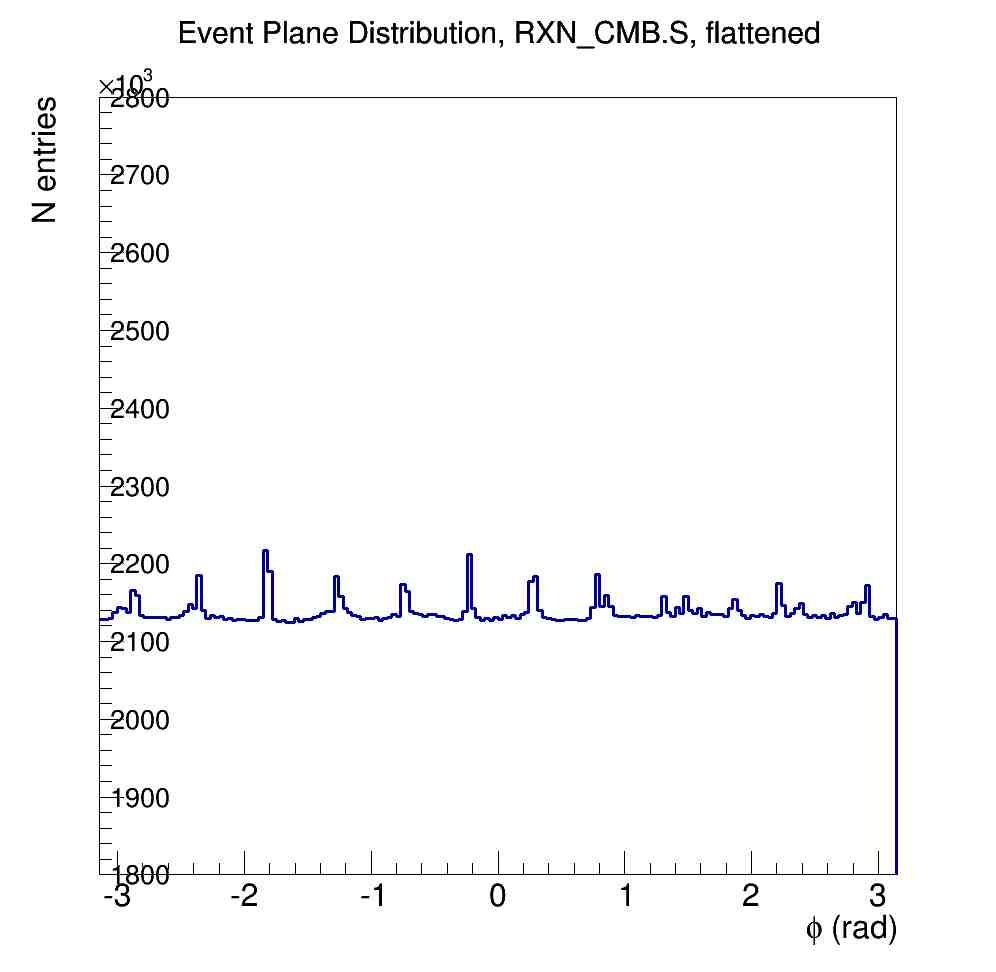
\includegraphics[width=1\textwidth]{EPflattening/flatrxncmbs.jpg}
    \end{subfigure}
    \rule{35em}{0.5pt}
  \caption[Flattened event plane distributions in the BBC, MPC, and RXNP]{Flattened event plane distributions in the BBC, MPC, and RXNP. Note that this flattening is significantly better in the ``gold-going'' south arm.}
  \label{fig:evtpln}
\end{figure}

Because the d+Au system is asymmetric by construction, track multiplicities on the north and south detectors are not the same. Rather, since gold ions have a considerably larger amount of nucleons than deuterons, it therefore has higher forward track multiplicity, and its event plane signature in the forward detectors is much stronger. In practice, the north side is the deuteron going side, and the south side is the gold going side. This can be seen clearly in figure \ref{fig:evtpln} where the event plane is much easier to flatten in the south than in the north regardless of which detector subsystem is chosen. I will be using the event plane as determined by the BBC in the south arm because of this and additionally because the event plane is flattest with it. However, additional independent measurements of the event plane are still useful as they can be used to correct resolution limitations.

\section{Event Plane Resolution Correction}
Since we have a finite number of readout channels in any of the chosen detectors capable of measuring the event plane, our track multiplicity distribution is not smooth and continuous, rather there is an associated resolution limitation for each measurement made with a specific detector. This resolution limitation affects how well we can measure flow anisotropies, and because of the nature and shape of various Fourier harmonics, higher harmonics are more strongly affected by resolution limitations since their shape is quickly varying over the azimuthal distribution compared to lower harmonics. Because of this, resolution corrections must be calculated for each harmonic separately. The apparatus make different measurements of the event plane using different Fourier harmonics and so the resolution corrections made for each detector are coupled to the Fourier harmonic used by the detector to find the event plane, that is to say, the Harmonic dependence and detector resolution dependence of the resolution correction are not separable. Additionally, by collision geometry, the ability to determine each correction is dependent on event centrality, implying that these corrections must be made for each centrality bin as well. The measured flow anisotropy decreases as the ability to resolve changes in flow decreases so we correct this resolution error by defining some multiplicative scaling such that:
\begin{equation}
v_n = \frac{v_n^{A}}{Res(\Psi_n^A)}
\end{equation}
where $v_n^{A}$ is the $n^{th}$ order anisotropic flow coefficient measured with some detector, arbitrarily designated A, and $Res(\Psi_n^A)$ is a single valued correction factor for the $v_n$ measurement using a specific detector and a single bin in centrality. Since device resolution is independent of particle species, we do not need to calculate a different correction for each particle flow. 

The method of determining resolution correction used for this analysis is called the \textit{Three Subevent Method} and can be calculated by comparing the event plane measured with one detector with measurements made by two other detectors, let's call the detector of interest: detector A, and the other two detectors B and C respectively. It can be shown \citep{PhysRevC.58.1671} that we can define this correction as:

%Specifically, we take a measurement of the event plane made by the detector whose resolution we would like to correct (say, detector A) and subtract a measurement of the same event plane made by another detector (detector B) take the cosine of two times that difference, i.e. $\langle cos(2k[\Psi^{A}-\Psi^{B}])\rangle$. This $cos (2 *\Delta \Psi)$ is chosen here since we are calculating the resolution correction for the 2nd harmonic. This gives us one approximation of the resolution correction but it is conceptually still dependent on the resolution limitations of detector B. We then take another approximation of the correction using a different detector (C) so we have the resolution limitation of detector A as measured by B and C. Then we can try to remove the dependence on B and C's resolution by dividing by another resolution approximation made using B and C's measurement. 
%----------------------------------------------------------------------------------------
\begin{equation}
Res\{n \Psi_n^{A}\} = \sqrt{\frac{\langle cos(n[\Psi_n^{A}-\Psi_n^{B}])\rangle \langle cos(n[\Psi_n^{A}-\Psi_n^{C}])\rangle}{\langle cos(n[\Psi_n^{B}-\Psi_n^{C}])\rangle}}
\end{equation} 
where $\Psi_n^X$ is the event plane as measured with detector X using the n$^{th}$ Fourier harmonic.
\pagebreak
\pagebreak
